\documentclass[../main.tex]{subfiles}

\begin{document}

\section{Materials and Methods}

\subsection{Microscopy}

A substantial amount of work for this project has been on determining the optimal microscopy technique for the live imaging of protein clustering.

The microscope used after trialling was as follows:

\begin{itemize}
\item{Nikon Eclipse Ti-E Inverted Microscope}
\item{40X 0.6NA long working distance plan objective}
\item{100X 1.49NA TIRF oil plan apo objective}
\item{Andor iXon 897 Ultra 512x512 pixel \SI{16}{\micro\meter} EMCCD camera}
\end{itemize}

An OptoSplit II system from Cairn Research was employed to visualise both channels of Homo- or Hetero- FRET measurements simultaneously. This unit is placed in the lightpath between the microscope and the camera. Within it, a dichroic and pair of filters project the same half of the image onto each half of the camera sensor in different wavelengths or polarisation orientations (Figure~\ref{fig:microscope}). It is also possible to block one light path and allow the other to fully occupy the camera sensor by means of adjusting mirrors and shutters.

Inside the OptoSplit II is a dichroic and two filters (one in the case of homo-FRET). Whilst there is already good wavelength filtering by the excitation and emission dichroics, the filters are required to clean up the signal and remove any longer wavelengths.

\paragraph{Excitation} was achieved with system described in Table~\ref{table:ledlighting}.

Only one blue wavelength (GFP or Blue) LED could be used at any one time. Lights from the back were combined sequentially with a \SI{515}{\nano\meter} and \SI{495}{\nano\meter} dichroic.

The white light for bright field has a red (\SI{590}{\nano\meter}) filter placed in front of it as the white LED requires a phosphorescent element to achieve the right spread of wavelengths. This phosphorescent element can be excited by fluorescence excitation, causing a high level of light to be reflected back through the lens and into the camera. The red filter blocks this transmission and allows for rapid switching between bright field and fluorescent excitation without having to block the light path.

For homo-FRET measurements, a rotating linear polariser could be inserted in front of the YFP LED (position (2)).

The entire microscope is mounted on a ThorLabs PerformancePlus Series II breadboard fitted to a ThorLabs Active Isolation frame. This was felt necessary due to the presence of noisy machinery in adjacent rooms, high foot traffic, and small size of the samples being observed (\(\sim\)\SI{2.5}{\micro\meter} in the largest dimension).

\paragraph{Emission} was controlled with the filters described in Table~\ref{table:filterset}.
\begin{figure}[p]
\begin{center}
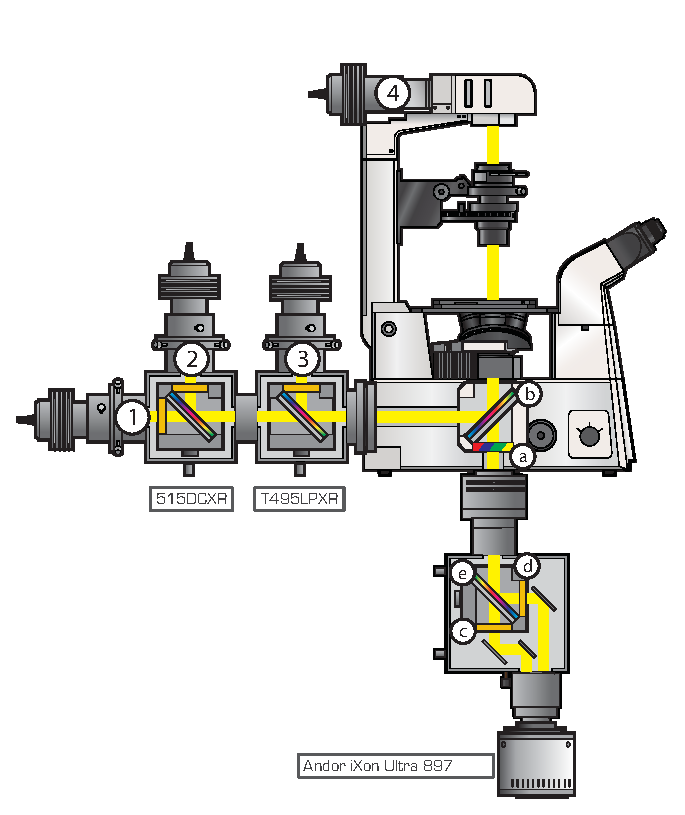
\includegraphics[scale=1]{\docroot matmeth/figs/microscope.eps}
\caption[Microscope schematic]{Microscope schematic. Whilst the camera is shown on bottom port of microscope for ease of presentation it is in fact mounted on the left port. Numbered locations are for LED/filter combinations, given in Table~\ref{table:ledlighting}. Lettered locations are for emission filters or dichroics,  given in Table~\ref{table:filterset}. The light from the LEDs in position 1 and 2 are combined by the dichroic 515DCXR, and then combined with the light from the LED in position 3 by the dichroic T495LPXR. Image generated using templates from Cairn Research.}
\label{fig:microscope}
\end{center}
\end{figure}
\begin{table}[p]
\begin{center}
\begin{tabular}{l|c|c|l}
\textbf{Fluorophore}	&	\textbf{LED wavelength}	&	\textbf{Filter}	&	\textbf{Location} \\\hline
mCherry	&	White	&	560/40x	&	(1)	\\
YFP		&	\SI{505}{\nano\meter}		&	500/20x	&	(2)\\
GFP		&	\SI{470}{\nano\meter}		&	470/40x	&	(3)\\
Blue		&	White	&	440/10x	&	(3)\\
Bright Field		&	White	&	\SI{590}{\nano\meter}	&	(4)
\end{tabular}
\caption[LED lighting system]{LED lighting system for microscope. White LEDs comprised LED and phosphorescent elements. Excitation filter specifications give central wavelength and width of filter, both in \si{\nano\meter}, with the x denoting excitation. GFP and blue illumination sources are interchangeable.}
\label{table:ledlighting}
\end{center}
\end{table}
\begin{table}[p]
\begin{center}
\begin{tabular}{l|c|c|c|c|c}
&	\multicolumn{2}{c|}{Filter Wheel}	&	\multicolumn{3}{c}{OptoSplit II}	\\
\textbf{Description}	&	\textbf{Dichroic} (b)	&	\textbf{Filter} (a)		& \textbf{Dichroic} (e)	&	\textbf{Filter} (d)	&	\textbf{Filter} (c)	\\\hline
mCherry	&	\SI{585}{\nano\meter}		&	630/75m	&	-	&	-	&	-	\\
YFP		&	\SI{515}{\nano\meter}		&	535/30m	&	-	&	-	&	-	\\
YFP homo-FRET	&	\SI{515}{\nano\meter}	&	535/30m	&	Polarising	&	Polarising	&	-	\\
YFP\(\rightarrow\)mCherry Fret	&	\SI{515}{\nano\meter}	&	-	&	\SI{565}{\nano\meter}	&	545/40m	&	630/75m	\\
GFP		&	\SI{495}{\nano\meter}		&	525/50m	&	-	&	-	&	-	\\
Bright field		&	-	&	-	&	-	&	-	&	-	
\end{tabular}
\caption[Microscope filter set]{Filter set. Emission filter specifications give central wavelength and width of filter, both in \si{\nano\meter}, with the m denoting emission.}
\label{table:filterset}
\end{center}
\end{table}


\subsection{Laboratory Techniques}

\subsubsection{Standard Protocols}
\paragraph{MiniPreps} were performed with either a Fermentas GeneJet kit for sequencing or boiling lysis protocol~\citep{boiling} for anything else.
\paragraph{PCR} was performed with Phusion\textregistered\xspace polymerase according to the scheme in Tables~\ref{table:pcr:mix} and~\ref{table:pcr:protocol}.

\begin{table}
\begin{center}
\begin{tabular}{l|cc}
	&	\textbf{Stock Concentration}		&	\textbf{Volume}	\\\hline
5X Hi-Fi reaction buffer	&	5X	&	\SI{10}{\micro\litre}\\
\ce{MgCl2}	&	\SI{25}{\nano\Molar}	&	\SI{3}{\micro\litre}\\
Template	 	&	-	&	\(\sim{\SI{50}{\nano\gram}}\)\\
Primer (each)		&	\SI{10}{\nano\Molar}	&	\SI{1}{\micro\litre}\\
Phusion\textregistered\xspace polymerase	&	\SI{2000}{\unit\per\milli\litre}	&	\SI{1}{\micro\litre}\\
Water	&	-	&	to make\\\hline
\textbf{Total}	&	-	&	\SI{50}{\micro\litre}
\end{tabular}
\caption[PCR Mix]{PCR Mix. As most of the templates were stored in the \SIrange{40}{80}{\nano\gram\per\micro\litre} range, \SI{1}{\micro\litre} was added. If they exceeded this, they were diluted by half before being added.}
\label{table:pcr:mix}
\end{center}
\end{table}

\begin{table}
\begin{center}
\begin{tabular}{lcc}
Initial Denaturation	& \SI{98}{\degreeCelsius} & \SI{120}{\second}\\
\multicolumn{3}{c}{\textbf{Loop 30 times:}}\\
Denaturation		&	\SI{98}{\degreeCelsius}		&	\SI{30}{\second}\\
Annealing 		&	Optimal for primer	&	\SI{30}{\second}\\
Extension		&	\SI{72}{\degreeCelsius}		&	\SI{30}{\second\per\kilo\base}\\
\multicolumn{3}{c}{\textbf{End Loop}}\\
Final extension	&	\SI{72}{\degreeCelsius}		&	\SI{7}{\minute}\\
Hold				&	\SI{4}{\degreeCelsius}		&	\(\infty\)
\end{tabular}
\caption{PCR Protocol}
\label{table:pcr:protocol}
\end{center}
\end{table}

\paragraph{Transformation} was performed on \ce{CaCl2} competent cells using a protocol modified from~\citet{transform}, then plated onto LB Agar plates with appropriate antibiotic.

\subsubsection{Chemicals}

Unless specified otherwise, chemicals were from Sigma Aldrich, of the highest grade available.

\subsubsection{Gibson Assembly}

Gibson Assembly can be performed in volumes from about \SIrange{5}{20}{\micro\litre}. Initially, larger volumes were used but as efficiency became apparent smaller volumes were used to economise. Roughly equimolar concentrations of gel purified overlapping DNA were added to the 1.33X Gibson Master Mix in a \SI{50}{\micro\litre} tube on ice. This was incubated for \SI{1}{\hour} at \SI{50}{\degreeCelsius}, before being returned to ice. \SIrange{5}{10}{\micro\litre} was then used to transform cells.

All protocols and buffers for Gibson Assembly are from~\citet{gibson09}.

\begin{table}
\begin{center}
\begin{tabular}{c|c|c}
&\textbf{Stock Concentration} (\si{\unit\per\micro\litre})&\textbf{Volume} (\si{\micro\litre})\\\hline
Taq ligase				&	40		&	50\\
5X Isothermal Buffer		&	5X		&	100\\
T5 Exonuclease			&	1		&	2\\
Phusion\textregistered\xspace Polymerase		&	2		&	6.25\\
Nuclease free water		&			&	216.75\\\hline
\textbf{Total}			&	1.33X	&	375
\end{tabular}
\caption[Gibson Master Mix]{Gibson Master Mix. This was prepared on ice in the Taq ligase tube, before being aliquoted into \SI{75}{\micro\litre} portions for freezing at \SI{-20}{\degreeCelsius}.}
\end{center}
\end{table}

\begin{table}
\begin{center}
\begin{tabular}{c|c|c}
&\textbf{Stock Concentration} (\si{\milli\Molar})&\textbf{Volume} (\si{\micro\litre})\\\hline
PEG-8000					&	25\%		&	\SI{0.75}{\gram}\\
Tris-\ce{HCl} pH 7.5		&	500		&	1500\\
\ce{MgCl2}				&	50		&	75\\
DTT						&	50		&	150\\
dATP						&	1		&	30\\
dTTP						&	1		&	30\\
dCTP						&	1		&	30\\
dGTP						&	1		&	30\\
NAD						&	5		&	300\\
Nuclease free water		&			&	...\\\hline
\textbf{Total}			&	5X		&	3000
\end{tabular}
\caption[5X Isothermal Buffer]{5X Isothermal Buffer. Prepared on ice and stored at \SI{-20}{\degreeCelsius}.}
\end{center}
\end{table}


\subsubsection{Preparation of Cells for Microscopy}

The following protocol was followed for preparing cells for microscopy.

\begin{enumerate}
\item Prepare \SI{2}{\milli\litre} overnight culture with appropriate antibiotic (\SI{100}{\micro\gram\per\milli\litre} ampicillin and/or \SI{34}{\micro\gram\per\milli\litre} chloramphenicol).
\item Inoculate \SI{20}{\micro\litre} overnight culture in \SI{2}{\milli\litre} fresh LB with appropraite antibiotic and inducer (\SI{25}{\micro\molar} IPTG or 0.01\% arabinose, unless stated otherwise).
\item Pellet the cells in a \SI{1.5}{\milli\litre} microcentrifuge tube for \SI{10}{\minute} at \SI{16000}{\grav}.
\item Aspirate off supernatant
\item Resuspend in \SI{500}{\micro\litre} PBS, with or without \SI{2}{\milli\Molar} \ce{CoSO4}.
\item \paragraph{If fixing}
\begin{enumerate}
\item Add \SI{12.5}{\micro\litre} 37-41\% formaldehyde to make 1\%.
\item Incubate for 10 minutes at room temperature.
\end{enumerate}
\item[] \paragraph{Then}
\item Spin down cells.
\item Resuspend in \SI{1}{\milli\litre} PBS.
\item Spin down cells.
\item Resuspend in \SI{500}{\micro\litre} PBS.
\end{enumerate}

The final resuspension volume was be adjusted to match cell density depending on mounting method. Initial volume was also be adjusted with corresponding changes to subsequent volumes. Concentration of \ce{CoSO4} was varied according to requirements.

\paragraph{STED} microscopy requires special cell preparation to help protect against bleaching. The following protocol was used from Jackson ImmunoResearch~\citep{jackson}:

\begin{enumerate}
\item Prepare and wash cells as above
\item Make up 90\% glycerol in 10X PBS
\item Make up 20\% w/v n-propyl gallate in dimethyl sulfoxide
\item Add 1/100 volume of 20\% NPG to 90\% glycerol/1x PBS dropwise with rapid stirring
\item Resuspend cells in \SI{500}{\micro\litre} of the above
\end{enumerate}

\paragraph{Cell Mounting} Cells were mounted on \#1.5 slides for imaging. Work is still ongoing to optimise a poly-L-lysine protocol to hold the cells in place.


\subsection{Image Processing}
\label{sec:method:imageproc}
Unless otherwise stated, all image processing has been done in MATLAB version 2011b. All processing scripts are open source and have been made publicly available, see section~\ref{sec:scripts:clusters}. Details of the process of the scripts are given in section~\ref{sec:results:imageprocessing}.

\subsection{MicroManager}

In order to give maximum flexibility, the microscope and all related equipment were controlled using MicroManager~\citep{micromanager}, an open source software package for control of microscope and associated devices. A beanshell driver was written for the syringe pumps to allow easy integration into experimental workflow, along with several scripts to run experiments. Latest versions of these may be found online, see section~\ref{sec:scripts:micromanager}.

\end{document}
